\section{Instrumentation}

\begin{itemize}

    \item[-] \textbf{Flute}, with shaker \\

    \item[-] \textbf{Oboe} \\

    \item[-] \textbf{Clarinet in b-flat}, with shaker \\

    \item[-] \textbf{Percussion} \\

        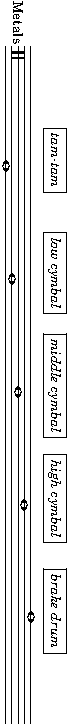
\includegraphics{../assets/preface-percussion-metals.pdf} \\ \\ \\
        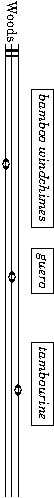
\includegraphics{../assets/preface-percussion-woods.pdf} \\ \\ \\
        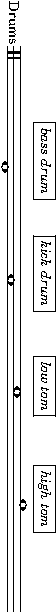
\includegraphics{../assets/preface-percussion-drums.pdf} \\

        Mallets: hard sticks or bare hands, wire brushes, superballs \\

    \item[-] \textbf{Piano} \\

        Prepare the strings in the lowest and highest octaves with any
        combination of felt, tape or rubber to dampen and distort the timbre of
        the strings. Putty-like substances work particularly well. \\

        Guero passages should be played with a piece of hard paper or
        plastic (e.g. a credit card), on the keys. 
        The register of the motions is left to the performer. \\

    \item[-] \textbf{Violin}, with shaker \\

    \item[-] \textbf{Viola}, with shaker \\

    \item[-] \textbf{Cello}

\end{itemize}

    Auxiliary shakers should be maracas, cabasas, brazil nut shakers or
    simliar. Uniform and disparate selections are equally interesting.
